\documentclass{article}
\usepackage{arxiv}

\usepackage[utf8]{inputenc}
\usepackage[english, russian]{babel}
\usepackage[T1]{fontenc}
\usepackage{url}
\usepackage{booktabs}
\usepackage{amsfonts}
\usepackage{nicefrac}
\usepackage{microtype}
\usepackage{lipsum}
\usepackage{graphicx}
\usepackage{natbib}
\usepackage{doi}



\title{Multiply learning in recommendation systems}

\author{ David S.~Hippocampus\thanks{Use footnote for providing further
		information about author (webpage, alternative
		address)---\emph{not} for acknowledging funding agencies.} \\
	Department of Computer Science\\
	Cranberry-Lemon University\\
	Pittsburgh, PA 15213 \\
	\texttt{hippo@cs.cranberry-lemon.edu} \\
	%% examples of more authors
	\And
	Elias D.~Striatum \\
	Department of Electrical Engineering\\
	Mount-Sheikh University\\
	Santa Narimana, Levand \\
	\texttt{stariate@ee.mount-sheikh.edu} \\
	%% \AND
	%% Coauthor \\
	%% Affiliation \\
	%% Address \\
	%% \texttt{email} \\
	%% \And
	%% Coauthor \\
	%% Affiliation \\
	%% Address \\
	%% \texttt{email} \\
	%% \And
	%% Coauthor \\
	%% Affiliation \\
	%% Address \\
	%% \texttt{email} \\
}
\date{}

\renewcommand{\shorttitle}{\textit{arXiv} Template}

%%% Add PDF metadata to help others organize their library
%%% Once the PDF is generated, you can check the metadata with
%%% $ pdfinfo template.pdf
\hypersetup{
pdftitle={A template for the arxiv style},
pdfsubject={q-bio.NC, q-bio.QM},
pdfauthor={David S.~Hippocampus, Elias D.~Striatum},
pdfkeywords={First keyword, Second keyword, More},
}

\begin{document}
\maketitle

\begin{abstract}
        This paper addresses the issue of evaluating the quality of recommender systems in the long term, taking into account the evolution of consumers and product assortments. We consider the dynamical system of changes in consumers and products over time. The main purpose of the study is to identify the conditions under which degeneracies in audience, assortment, or transaction distribution occur in a given repeated machine learning system, and how such phenomena depend on the learning algorithms and recommendation models. Using the obtained results, we can present a model that is able to increase the metrics in the recommendation systems without degenerating the distributions on products and customers. We conduct a series of computational experiments on the synthetic datasets, the results of the experiments correspond to the theoretical predictions derived from the dynamical model
\end{abstract}


\keywords{Repeated Machine Learning \and Feedback loop}

\section{Introduction}
Recommender systems are an important component of many online services, such as search engines, e-commerce platforms, news services, and social networks. They are very convenient tools because their main task is to offer users the most relevant items based on the available information. Modern recommender system models are adaptable to users, but it is also true that recommender systems influence user behavior. This work explores the problem of multiple training in recommender systems. Multiple training refers to a machine learning method in which data becomes available sequentially and is used to improve predictions for subsequent data.

The importance of recommender systems is supported by numerous studies[2, 3]. In multiple training models, unexpected effects can arise, leading to suboptimal results. For example, excessive personalization can trap users in so-called "filter bubbles," increasing user bias[1]. Also, in multiple training, "feedback loops" can occur, calling into question the quality of recommendations[4]. Another effect that arises in multiple training is the degeneration of the distribution of original items[5]. We specifically address this issue in the recommender system model and aim to propose an algorithm to prevent it.

Existing literature explores various methods for solving similar problems, emphasizing the complexity of optimizing recommendation metrics while ensuring stability in distribution patterns over time. One of the main focuses of our research is feedback loops resulting from user interaction with the recommender system. Previously, the problem was approached from a different angle, describing how to overcome input data bias to improve the algorithm[8]. Some sufficient conditions have also been identified for when a dynamic system with multiple training leads to distribution degeneration[9].

In this article, we propose a new mathematical model for the process of mupltiply learning in recommender systems not previously discussed in the literature. Our goal is to propose an algorithm that improves known metrics for recommender algorithms, such as nDCG, RMM, map@K [6,7], while preventing the degeneration of user and item distributions.

\section{Problem statement}

Рассмотрим модель динамической рекоммендательной системы. Пусть $C$ - множество покупателей, $W$ --- множество товаров, $|C|, |W| < \infty$. Покупатели $c$ и товары $w$ описываются конечным числом признаков, то есть $ c \in C \subset \mathbb{R}^d, w \in W \subset \mathbb{R}^l$. На каждом шаге $t$ имеется распределения с плотностями $f_c^t$ и $f_w^t$ на множествах $C$ и $W$ соответственно, при $t = 0$ оба распределения известны. Данные функции отражают распределения признаков среди покупателей и товаров в системе. В последствии эти распределения будут меняться в процессе работы системы. Эти изменения отражает оператор эволюции $\text{D}_t : \textbf{R}_d \times \textbf{R}_l \rightarrow R_d \times R_l $, где $R_k$ --- множество всех функций плотности на $\mathbb{R}^k$. Таким образом, $(f_c^{t + 1}, f_c^{t+1}) = \text{D}_t(f_c^{t}, f_c^{t})$.\\
Цель работы --- предложить алгоритм, который улучшает стандартные метрики для рекомендательных алгоримтов (p@K, map@K, nDCG, MRR) при условии, что в пределе не возникает вырождения распределения товаров и пользователей. Под вырождением распределения покупателей имеется в виду, что $ f_c^t \rightarrow f_c $, где носитель $ f_c $ --- подпространство $ \mathbb{R}^d $ меньшей размерности. Аналогично определяем вырождение для распределения товаров. Для объяснения того, что подразумеваеся под улучшением метрик, введем понятие "невязок". Пусть на шаге $t$ модель по данным X предсказывает рекомендации $y_{pred} = H(X, t)$, $y_{true}$ --- предпочтения пользователей в действительности, тогда вектором невязок будем называть $y_{pred} - y_{true}$. Есть следующие свойства: \\
1) || $y_{pred} - y_{true}$ || --- маленькое число $\Leftrightarrow$ метрики большие.\\
2) невязка может иметь отрицательные компененты. \\
Таким образом, условие улучшения стандартных метрик сводится к минимизации норм векторов невязок. Достаточным условием для этого в пределе будет являться выполнение следующего условия: $y_{pred} - y_{true} \xrightarrow{t \rightarrow \infty } \delta$, где $\delta$ --- дельта-функция Дирака. \\
Теперь рассмотрим конкретный пример динамической системы. Пусть имеется функция $\mu_t: C \times W \rightarrow [0, 1] $ --- агрегированный фидбек для каждой пары из товара и пользователя за время работы системы, $\mu_0(c, w) = 0\ \forall c, w$. Теперь опишем одну итерацию в модели работы динамической системы:
\begin{enumerate}
\item Происходит сэмплирование выборок произвольного размера покупателей и товаров из распределений $f_c^t$ и $f_w^t$:
$c_1^t,..,c_n^t \sim f_c^t,\ w_1^t,..,w_k^t \sim f_w^t$.
\item Рекомендательная система подбирает для каждого покупателя из выборки подмножество товаров из $w_1^t,..,w_k^t$
\item Покупатели совершают покупку с вероятностью $u(c, w)$, где $u : C \times W \rightarrow [0, 1]$ --- фиксированная функция полезности товара для данного пользователя. Далее рекоммендательная система дообучается на полученном фидбэке, используя базовый алгоритм рекомендательный системы.
\item Шаги 2-3 повторяются произвольное количество раз.
\item Обозначим за $M_{t+1}$ --- набор фидбэков, полученных за все повторения шага 3 на данной итерации, то есть мультимножество из троек вида $(c, w, m)$, где $c \in {c_1^t,..,c_n^t},\ w \in {w_1^t,..,w_k^t},\ m \in \{0, 1\}$, где 1 обозначает совершение покупки, 0 --- её отсутствие. Далее обновляется функция $\mu_t$. Пусть сначала $\mu_{t + 1} = \mu_t$. Далее для каждой тройки $(c, w, m)$ из $M_{t+1}$ функцию $\mu_{t + 1}$ изменяется так: $\mu_{t + 1}(c, w) = \lambda m + (1 - \lambda)\mu_{t}(c, w)$, где $\lambda \in [0, 1]$ --- некоторая константа, отражающее скорость забывания старого фидбэка.
\item Далее проиходит обновление распределений товаров и пользователей в соответствии с новой функцией $\mu_{t + 1}$. Будем это делать при помощи сглаживания Лапласа:
$f_w^{t+1}(w_i) = \frac{\sum_{c \in C} (\mu_{t + 1}(c, w_i) + \delta)}{\sum_{w \in W, c \in C} (\mu_{t + 1}(c, w) + \delta)}$, где $\delta > 0$ --- небольшая константная поправка. Поправка используется для того, чтобы ещё ни разу не показанные товары всё ещё попасть в систему с ненулевой вероятностью. Аналогично обновляется $f_c^{t+1}$.
\end{enumerate}

\subsection{Headings: second level}
\lipsum[5]
\begin{equation}
	\xi _{ij}(t)=P(x_{t}=i,x_{t+1}=j|y,v,w;\theta)= {\frac {\alpha _{i}(t)a^{w_t}_{ij}\beta _{j}(t+1)b^{v_{t+1}}_{j}(y_{t+1})}{\sum _{i=1}^{N} \sum _{j=1}^{N} \alpha _{i}(t)a^{w_t}_{ij}\beta _{j}(t+1)b^{v_{t+1}}_{j}(y_{t+1})}}
\end{equation}

\subsubsection{Headings: third level}
\lipsum[6]

\paragraph{Paragraph}
\lipsum[7]



\section{Examples of citations, figures, tables, references}
\label{sec:others}

\subsection{Citations}
Citations use \verb+natbib+. The documentation may be found at
\begin{center}
	\url{http://mirrors.ctan.org/macros/latex/contrib/natbib/natnotes.pdf}
\end{center}

Here is an example usage of the two main commands (\verb+citet+ and \verb+citep+): Some people thought a thing \citep{kour2014real, hadash2018estimate} but other people thought something else \citep{kour2014fast}. Many people have speculated that if we knew exactly why \citet{kour2014fast} thought this\dots

\subsection{Figures}
\lipsum[10]
See Figure \ref{fig:fig1}. Here is how you add footnotes. \footnote{Sample of the first footnote.}
\lipsum[11]

\begin{figure}
	\centering
	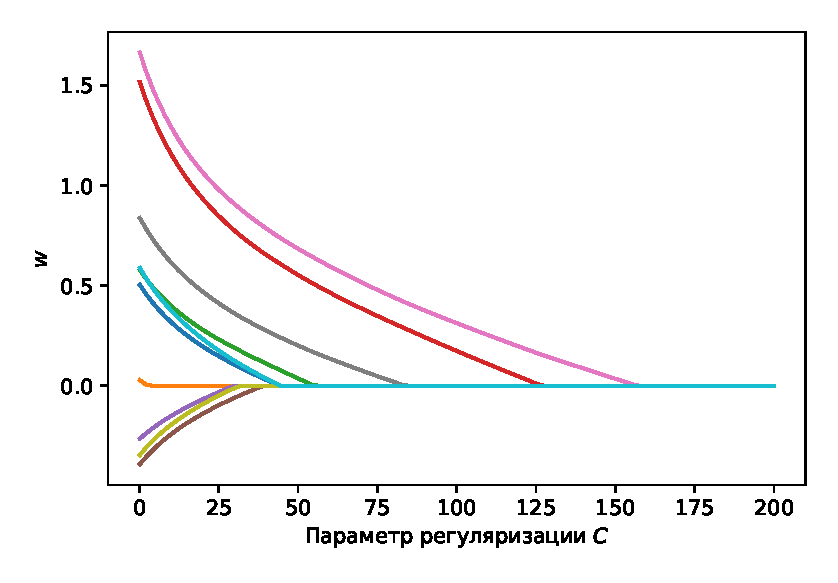
\includegraphics[width=0.5\textwidth]{../figures/log_reg_cs_exp.eps}
	\caption{Sample figure caption.}
	\label{fig:fig1}
\end{figure}

\subsection{Tables}
See awesome Table~\ref{tab:table}.

The documentation for \verb+booktabs+ (`Publication quality tables in LaTeX') is available from:
\begin{center}
	\url{https://www.ctan.org/pkg/booktabs}
\end{center}


\begin{table}
	\caption{Sample table title}
	\centering
	\begin{tabular}{lll}
		\toprule
		\multicolumn{2}{c}{Part}                   \\
		\cmidrule(r){1-2}
		Name     & Description     & Size ($\mu$m) \\
		\midrule
		Dendrite & Input terminal  & $\sim$100     \\
		Axon     & Output terminal & $\sim$10      \\
		Soma     & Cell body       & up to $10^6$  \\
		\bottomrule
	\end{tabular}
	\label{tab:table}
\end{table}

\subsection{Lists}
\begin{itemize}
	\item Lorem ipsum dolor sit amet
	\item consectetur adipiscing elit.
	\item Aliquam dignissim blandit est, in dictum tortor gravida eget. In ac rutrum magna.
\end{itemize}


% \bibliographystyle{unsrtnat}
% \bibliography{references}

[1] Dominic Spohr. Fake news and ideological polarization: Filter bubbles and selective exposure on social media. \newline
[2] Billsus, Daniel & Pazzani, Michael. (2003). User Modeling for Adaptive News Access. User Modelling and User-Adapted Interaction. 10. 10.1023/A:1026501525781.\newline
[3] Pedreschi, D. and Miliou, I. and European Parliament. Directorate-General for Internal Policies of the Union Artificial Intelligence (AI): new developments and innovations applied to e-commerce European Parliament, 2020.\newline
[4] Krauth K., Wang Y., Jordan M. I. Breaking feedback loops in recommender systems with causal inference //arXiv preprint arXiv:2207.01616. – 2022.\newline
[5] Khritankov, Anton. 2023. “Positive Feedback Loops Lead to Concept Drift in Machine Learning Systems.” Applied Intelligence 53 (19): 22648–66. https://doi.org/10.1007/s10489-023-04615-3.\newline
[6] Yongfeng Zhang, Xu Chen, Qingyao Ai, Liu Yang, and W. Bruce Croft. 2018. Towards Conversational Search and Recommendation: System Ask, User Respond. In Proceedings of the 27th ACM International Conference on Information and Knowledge Management (CIKM '18). Association for Computing Machinery, New York, NY, USA, 177–186. https://doi.org/10.1145/3269206.3271776\newline
[7] Wang, Y., Wang, L., Li, Y., He, D. &amp; Liu, T.. (2013). A Theoretical Analysis of NDCG Type Ranking Measures. <i>Proceedings of the 26th Annual Conference on Learning Theory</i>, in <i>Proceedings of Machine Learning Research</i> 30:25-54 Available from https://proceedings.mlr.press/v30/Wang13.html.\newline
[8] Krueger, D., Maharaj, T., & Leike, J. (2020). Hidden incentives for auto-induced distributional shift. arXiv preprint arXiv:2009.09153.

\end{document}
